\chapter{系统总体设计}
本章对数字化运营平台进行总体设计。先分析了系统的整体架构与分层职责；随后对平台功能模块进行划分，明确本文负责实现的核心功能范围，为后续详细设计与系统实现提供依据。

\section{系统整体架构设计}
数字化运营平台面向企业内部多个部门的项目管理人员和运营团队，使用人员分布在研发、测试和管理等多个岗位，日常办公终端环境存在差异。平台在上线后需要根据业务变化持续迭代功能，对版本发布和升级的便捷性有一定要求。为降低客户端安装、升级和版本维护成本，本文延续 B/S 架构进行设计与开发，用户只需通过浏览器即可访问系统，能够降低终端适配和版本管理的复杂度。

为了降低模块之间的耦合度，并提高系统后续维护和扩展的便利性，本文在整体架构设计中采用分层设计思想，将系统划分为前端展示层、请求处理层、业务逻辑层、数据访问层和数据层五个部分\cite{iso42010_2022}。各层之间按照相对明确的调用关系进行协作，上层主要负责展示结果和接收请求，下层则负责业务处理、数据访问和数据持久化。

具体而言，展示层由前端页面组成，负责用户交互、数据展示和请求发送；请求处理层负责对请求进行身份和权限校验；业务逻辑层负责处理项目管理、公司运营管理等核心业务规则；数据访问层负责封装对数据库的访问操作；数据层则用于保存系统运行过程中产生和同步的业务数据。通过这种分层方式，系统的页面展示、业务处理和数据操作能够保持相对独立，有利于提高系统结构的清晰度。系统整体架构如图~\ref{fig:system-architecture} 所示。
\begin{figure}[htbp]
	\centering
	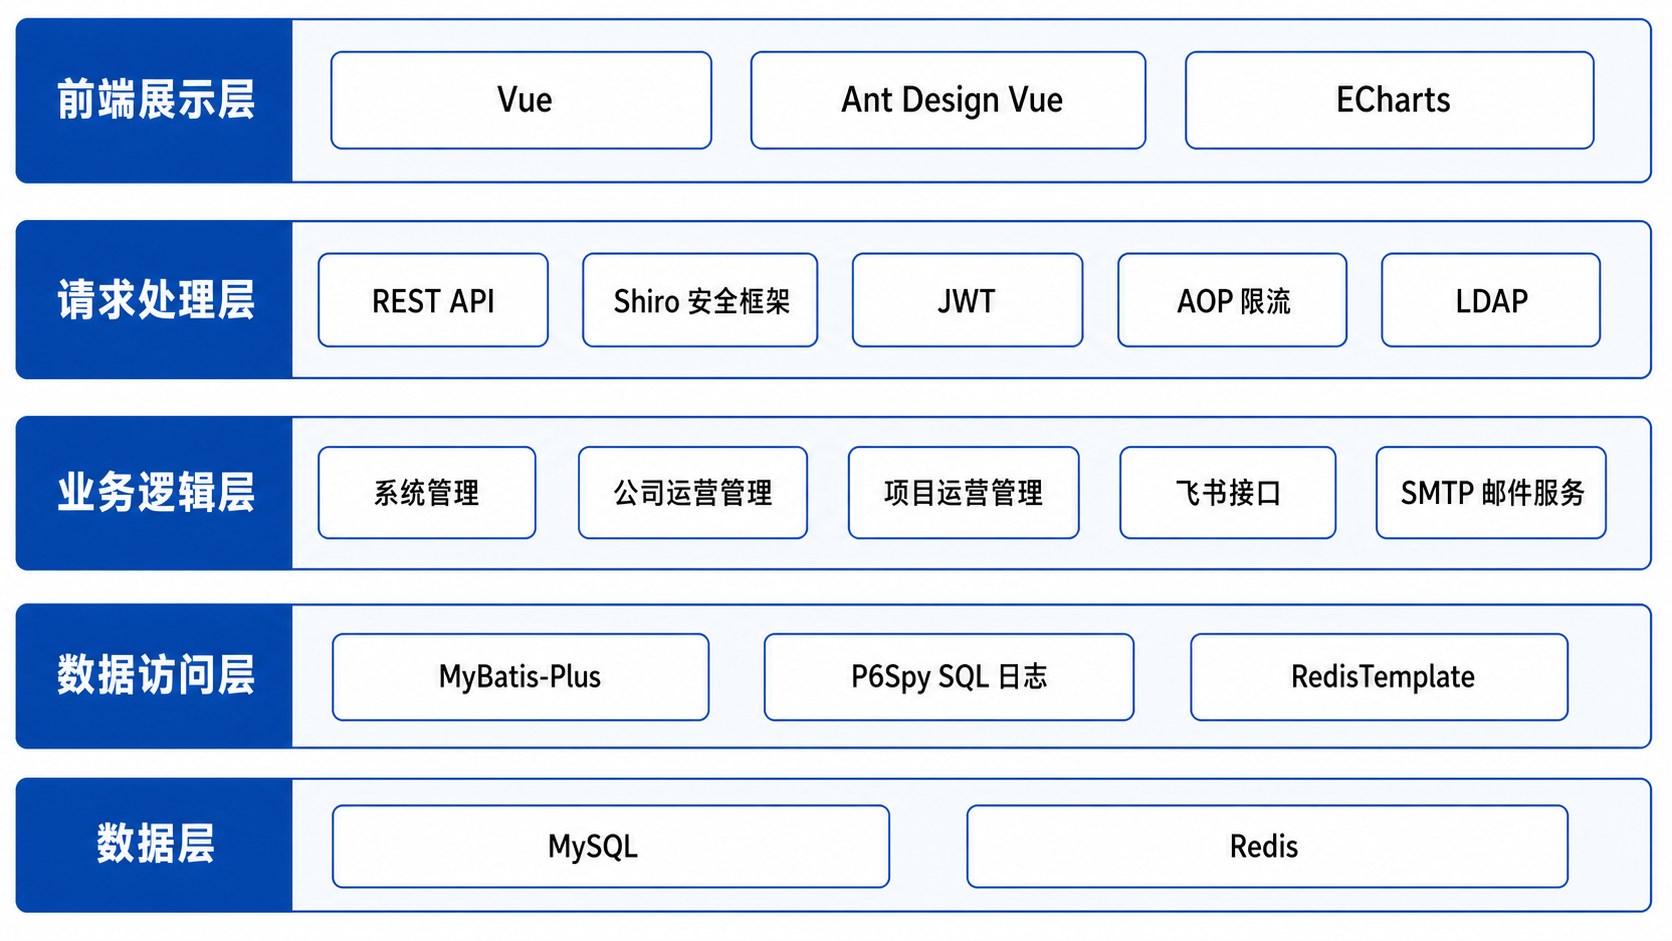
\includegraphics[width=1.0\linewidth]{imgs/arch/系统架构图2.png}
	\caption{系统架构图}
	\label{fig:system-architecture}
\end{figure}

第一层为\textbf{前端展示层}。
负责系统页面展示、用户交互和数据可视化等工作。本系统前端基于 Vue 进行开发，页面组件和基础交互控件主要采用 Ant Design Vue 实现，能够满足表单、表格、按钮、弹窗等后台管理系统常见界面的开发需求。对于数据展示场景，系统使用 ECharts 绘制柱状图、折线图、饼图等可视化图表，使用户能够更直观地理解统计结果。前端通过 Axios 与后端接口进行 HTTP 通信，然后从后端返回的 JSON 格式中拿到数据。前端项目运行环境依赖 Node.js，并通过 npm 管理前端依赖，使用 Webpack 完成项目打包和构建。

第二层为\textbf{请求处理层}。
位于前端界面和后端业务处理之间，主要负责身份认证、权限校验和接口访问控制，作为后端服务的统一“过滤器”。本系统使用 Shiro 安全框架实现用户认证与授权管理，通过 JWT（JSON Web Token）在用户登录后颁发身份令牌，前端在访问登录接口后拿到令牌并保存到本地，后续所有请求都在请求头中携带该令牌，后端对令牌有效性和用户权限进行校验。用户登录时，系统结合 LDAP（Lightweight Directory Access Protocol）进行企业内部的统一身份认证。除身份和权限控制外，系统还通过 AOP 自定义注解方式对部分接口进行限流处理，避免短时间内重复请求对系统造成过大压力。

第三层为\textbf{业务逻辑层}。
该层是系统后端的核心部分，主要负责项目管理、公司运营管理等业务功能的处理。前端发起的 HTTP 请求在通过安全校验后，会根据请求方式和请求路径分发到对应的后端接口，并进入具体的业务模块。
在业务处理过程中，系统首先对请求参数进行必要的校验，保证输入数据符合接口处理要求。对于部分统计类或查询频率较高的数据，业务逻辑层会优先判断缓存中是否存在有效结果；若缓存命中，则直接返回缓存数据，减少重复计算和数据库访问；若缓存中不存在有效数据，则继续执行相应的业务规则处理、数据统计计算和结果封装等操作。业务逻辑层在需要访问数据库时，会调用数据访问层提供的数据访问方法。最终，业务逻辑层将处理结果封装为统一的响应对象，并返回给前端展示。

第四层为\textbf{数据访问层}。
数据访问层负责屏蔽底层数据读写细节。MyBatis-Plus 提供基础的数据访问能力，但是由于过度封装，相比于传统的 XML 手写SQL来说并不是很直观。为了满足查看SQL执行计划的需要，使用P6Spy SQL 日志用于记录和分析 SQL 执行情况，RedisTemplate 用于操作缓存数据。业务逻辑层不直接访问数据库，而是通过这一层提供的接口完成数据查询和写入。

第五层为\textbf{数据层}。
数据层负责系统数据的持久化和缓存支撑。MySQL 存储系统权限、用户、项目、缺陷、运营等核心业务数据；Redis 用于缓存、会话和高频访问数据，提升热点数据查询的响应速度并减轻数据库压力。

\section{系统功能模块划分}
在上述分层架构的基础上，从业务维度对后端工程进行功能模块划分，将系统拆分为三个核心业务域：系统管理、公司运营管理和项目运营管理，以降低模块间的耦合度并提升代码的可维护性。从整体功能上看，项目管理模块主要围绕汽车电子软件过程管理展开，包括项目基础信息、缺陷、重大问题、风险、版本范围等功能；公司运营管理模块主要面向企业组织、员工、工时和KPI等运营数据，支持企业内部运营情况的统计分析；系统管理模块主要包括用户管理、角色管理、菜单管理、系统监控和日志管理等功能，用于保障系统的正常运行。

其中，项目管理和公司运营管理承担主要业务功能，系统管理为业务模块提供用户、权限和菜单等基础支撑。本文根据毕业设计任务分工，重点对其中部分功能模块进行设计与实现，包括公司运营管理下的部门投入 BU 工时分布，项目运营管理下的项目基本信息管理、缺陷管理和重大问题管理，如图\ref{fig:function-module}所示。
\begin{figure}[htbp]
	\centering
	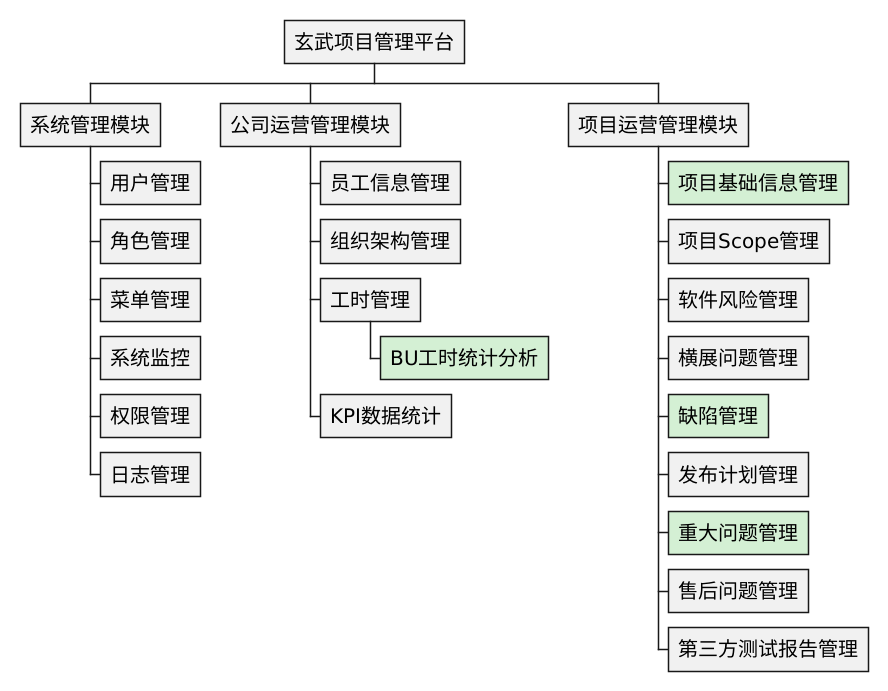
\includegraphics[width=0.7\linewidth]{imgs/玄武功能模块图Detail.png}
	\caption{系统功能模块划分图}
	\label{fig:function-module}
\end{figure}

(1)部门投入BU工时分布

主要用于从部门维度统计各业务单元的工时投入情况。该功能面向管理人员对部门资源投入结构的分析需求，通过对工时数据、员工信息和组织信息进行关联汇总，展示指定部门在不同 BU 方向上的工时分布情况，从而帮助管理人员了解部门人力资源在各业务方向上的投入比例和变化趋势。该功能是部门经理使用的，前端每次发送的请求都会先经过请求处理层看看用户携带的 Token 是否有效，之后会解析出用户的ID,然后通过系统管理模块下的权限校验功能去数据库中查询该用户是否具备权限。
\clearpage

(2)项目基本信息管理

项目基本信息管理主要面向项目经理使用，用于对项目基础数据进行查询和维护，内容包括项目名称、项目类型、所属 BU、里程碑计划、平台、客户以及项目状态等信息。对于项目信息在运行过程中的变更，系统会保留相应的历史记录，从而保证项目数据的可追溯性。该模块也为其他业务功能提供基础数据支撑。例如，在 BU 工时分布中，为满足数据库范式要求，工时数据不会记录项目属于哪个业务单元，还需要关联项目信息表来查询。在新增风险、重大问题时，表单中的下拉框数据也需要使用该模块的接口来查询。

(3)缺陷管理

缺陷管理模块主要用于对项目缺陷数据进行查询、统计和导出，帮助质量人员掌握项目质量状态。这些缺陷数据来自于系统使用的 Trinity、BugClose、Jira 这三个缺陷管理平台，会通过定时任务同步到本地的数据库中。用户可以对缺陷数据进行分页查询，也可以将多个项目看作一个聚类来进行汇总分析。对于健康度较低的项目聚类，质量人员可以发送飞书消息提醒，这里就需要通过组织架构管理和员工信息管理模块的接口来确认消息的接收人员列表。此外，一个缺陷被发现并修复后，可能也会在其他项目中暴露，项目经理可以标记缺陷为需要横展，之后进入横展问题管理模块的流程。

(4)重大问题管理

重大问题管理模块主要用于对项目管理中比较严重的问题进行跟踪和处理。质量人员可以在该模块中维护重大问题的基本信息、责任人、所属项目、客户及处理进展等内容。对于新增或需要重点关注的问题，系统支持通过飞书消息进行通知，使相关责任人能够及时接收到问题信息并开展处理。重大问题可能由风险转入，也可能由横展引发。对一个重大问题，项目经理同样可以标记为需要横展，进入横展的流程。

\section{本章小结}
本章主要对数字化运营平台进行了总体规划与设计。首先从分层角度阐述了系统的五层架构，包含前端展示层、请求处理层、业务逻辑层、数据访问层与数据层，并标注了各层的核心技术栈选型。随后，从实际业务维度出发，将系统拆分为系统管理、公司运营管理和项目运营管理三大核心模块，并简要介绍了本文负责的功能模块主要职责。

